\documentclass[11pt, a4paper,twocolumn]{article}
\linespread{1.3} % 1.5 spacing
\usepackage{amsmath}
\usepackage[margin=0.5in]{geometry}
\usepackage{graphicx}

\title{\textbf{Control Systems - ELEN90055} \\ \textit{Workshop 4}}
\date{2018\\ Semester 1}
\author{George Juliff -- 624946\\ Kweku Acquah -- 741573\\Thomas Miles -- 626263}




\begin{document}
\maketitle
\pagenumbering{gobble}
\clearpage
\pagenumbering{arabic}
\section{Introduction}\label{sec:intro}
This project aims to create a feedback controller in order to balance an activated inverted pendulum in an upright position whilst rejecting various disturbances.

To achieve this goal, Simulink was used to interface with the robot the pendulum was mounted on, adjusting the controller configuration and parameters, sending commands, and receiving encoder data from the robot's motors as well as data from a gyroscope mounted on the pendulum. This allowed a wide range of variables to be tested to systematically assess their impact on the system behaviour, aiding in design decisions when choosing the final controller configuration.

%-----------------------------------------------------------------------------------------------------------------------------%
\section{	System Modelling	}\label{sec:model}

\subsection{	Building the Inverted Pendulum Model	}
	The model of the actuated inverted pendulum mounted on the LEGO MINDSTORMS EV3 robot was developed using a combination of physical reasoning from the mathematical model of the system, presenting the form of the model, and experimental data, to identify and approximate suitable model parameters.
Our aim was to identify and develop a suitable model to implement feedback control on the actuated inverted pendulum to balance the pendulum in the presence of disturbance – impulse disturbance from manually displacing the pendulum and disturbance introduced from the motion of the robot. For this reason, we expect this model to be a simplification of the real system and to inherently differ from the actual system in parameter values. Nonetheless, this model will resemble the actual system in form and will be sufficient to implement feedback control on the inverted pendulum.

\subsection{	Mathematical Model of the Inverted Pendulum		}
The mathematical basis for the inverted pendulum model is taken from ELEN90055 Problem Set 1. Figure \ref{fig:diagram} below shows a simplified inverted pendulum system:

\begin{figure}[h!]
\centering
\caption{Inverted Pendulum and DC Motor Systems}
\label{fig:diagram}
\end{figure}

In this model, only the ordinary differential equation (ODE) involving the mechanics of the system will be considered. This is because the experimental data obtained was from an unactuated system - only the mechanical dynamics of the system influenced this data. In this system:
\begin{itemize}
	\item $J = (J_m + ml^2)$: moment of inertia of the motor and load relative to the motor shaft (kg.m2)
	\item $b$: viscous damping of shaft ($N.s/m$)
	\item $\theta$: angular displacement of the motor shaft (rad)
\end{itemize}

\begin{figure}[h!]
\centering
\caption{Pendulum Model}
\label{fig:pend}
\end{figure}

Using the Newton-Euler equation for the angular acceleration of the pendulum about the motor shaft, we obtain the following equations:
\begin{align*}
	M &= J\ddot{\theta}	\\
	mgl\sin(\theta)-T_{damping} &= (J_m + ml^2)\ddot{\theta}\\
	mgl\sin(\theta) - b\dot\theta &= (J_m+ml^2)\ddot{\theta}\\
	mgl\sin(\theta) &= (J_m + ml^2)\ddot{\theta} + b\dot\theta\\
	\intertext{Assuming small values for theta:}\\
	\Rightarrow mgl\sin(\theta) + b\dot\theta &= (ml^2)\ddot{\theta} \qquad \text{(1)}\\
\end{align*}

Equation (1) is the ODE governing the free motion of the pendulum after displacement. As can be noted from the form of the expression, the frictional torque due to damping is additive. This choice yields a solution set which most closely resembles the solution set obtained from experimental data in the next section.

\subsection{	Experimental Data vs Calculated Data	}

	Experimental data obtained from displacing the pendulum as shown in Figure \ref{fig:free_pend} where the initial conditions were $ \dot{\theta}(0) = 0 $ and $ \theta(0) = \frac{\pi}{2} $ produced the figure below:

\begin{figure}[h!]
\centering
\caption{Free Pendulum Results}
\label{fig:free_pend}
\end{figure}
%TODO was it entirely trial and error ?
By trial-and-error, the following parameter values for $m$, $l$, and $b$ were chosen to obtain a suitable ODE solution set:
\begin{align*}
	m &= 0.20\quad \text{ Kg}\\
	l &= 0.11\quad \text{ m}\\
	b &= 0.004\quad \text{N.s/m}
\end{align*}
where $ g = 9.81 \text{ m}/\text{s}^2 $. These values yield the model shown in Figure \ref{fig:damping_match}
\begin{figure}[hb!]
\centering
\caption{Matching Model to Experimental Results}
\label{fig:damping_match}
\end{figure}
%TODO Explain the fuckery with the gyro, and account for it to maybe show a nicer figure.
	Figure \ref{fig:damping_match} clearly shows that the parameter values selected do not accurately represent the physical system. There is a clear error between the data obtained from the gyro sensor and the data obtained from solving the ODE. However, because the form of calculated model is like the experimental data, we can be confident that developing a controller which meets the provided specifications based on this model will produce a control action suitable for controlling and responding to the dynamics of the physical system.
Using the parameter values obtained we can now consider the actuated inverted pendulum system. A relevant subset of the stalled and no-load characteristics of the motor and a small-signal linearized approximation of are shown below:
%
\begin{align*}
	ml^2\ddot{\theta} &= \tau - b\dot{\theta} + mgl\theta \\
	\intertext{ where }	\\
	\tau &= \frac{Kt}{R}(v - K_b\dot{\theta}) \text{and}	\\
	\frac{K_t}{R} &= 1.66 \times 10^-2 \frac{N.m}{V}				\\
	K_b &= 0.297 \frac{\text{V}\cdot \text{sec}}{\text{rad}}\\
\end{align*}
%TODO care plagarism/paraphrase better
	Taking the Laplace Transform of the small-signal linear approximation and accounting for the "percentage full power" units 	of the motor command (percentage of 9 V) and gyro sensor and motor encoder angle measurement units (in degrees) yields the following transfer function between the motor command and pendulum angle in degrees:
\begin{align*}
	G(s) &= \frac{\Theta_{deg}(s)}{V_\%(s)} \qquad \frac{\text{degrees}}{\text{\% full power}}	\\
	\Rightarrow G(s) &= \frac{9}{100}\cdot \frac{180}{\pi}\cdot \frac{\frac{K_t}{R}}{(s^2 \times ml^2 + s \times (b+ \frac{K_t 					K_b}{R}) - mgl)} \\
\intertext{
	Substituting the system parameters yields the model we used to develop our controller: 
}
	G(s) &= 0.086090\cdot 00242 s^2+ 0.008959 s - 0.2158
\end{align*}

%-----------------------------------------------------------------------------------------------------------------------------%
\section{	Controller Design	}\label{sec:design}

	\subsection{	Performance Requirements	}
	The controller should:
	\begin{enumerate}
	\item Reject impulsive and step disturbances, imparted by manual displacement of the pendulum and turning the robot caused by the drive wheels respectively.
	\item Be internally stable.
	\item Have a phase margin of 40$^\circ$ or more.
	\item Have a complimentary sensitivity function bandwidth of less than 50 rad/sec.
	\end{enumerate}
	
	\subsection{	Controller Implementation	}

	% Controller equasion used
	% Brief overview of the type implemented and why it was chosen
	The controller used to achieve these requirements was a phase lead controller, of the form:
	\begin{center}
		$ C(s) = 100 \cdot \cfrac{(0.1s + 1)}{0.001s + 1} $
	\end{center}
		\begin{figure}[h!]
			\centering
			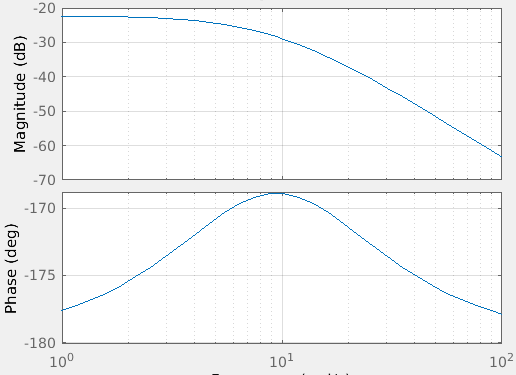
\includegraphics[scale=0.4]{bode_plant}
			\caption{Bode Plot of Plant Model}
			\label{fig:bode_plnt}
		\end{figure}
	\paragraph{		Model Considerations to Meet Requirements }
		
	\begin{itemize}
		\item \textit{Meeting the phase requirement}. Observing the phase part of Figure \ref{fig:bode_plnt}, it can be seen that to achieve the required phase margin the controller needs to add phase at crossover.
		\item \textit{Internal stability}. Figure \ref{fig:rl_plnt} shows the root locus plot of the plant transfer function detailed in section \ref{sec:model}. Because the model contains an unstable pole, sufficient gain to stabilise it must be used. Since the relative degree of the model is two, during controller design care was taken to avoid excessive gain values which develop undesirable oscillations in the system.
	\end{itemize}				
		
		\begin{figure}[h!]
			\centering
			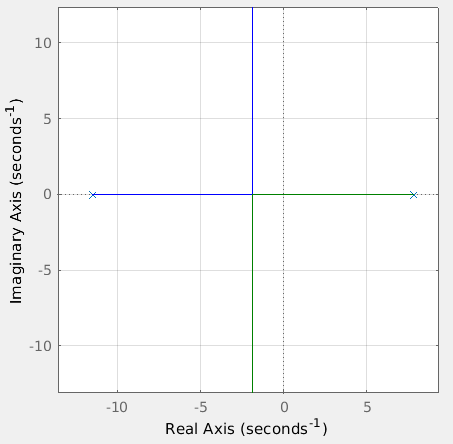
\includegraphics[scale=0.4]{rlocus_plant}
			\caption{Root Locus of Plant Model}
			\label{fig:rl_plnt}
		\end{figure}
						
			
	\paragraph{		Loop Shaping\\		}
			% Bode plot of plant, note what the controller needs to do to meet phase and gain spec
			% As such, explain how the choice of pole/zero placement generated desired results using bode/rlocus/nyquist
			The zero used in the controller was chosen to be placed between the poles in the plant model, this serves to completely stabilise the unstable pole in the plant for sufficiently high K. Since we want the crossover frequency of the complimentary sensitivity function $T_0$ to be less than 50 rad/sec. Figure \ref{} shows the phase increase resulting from placing the pole further from the origin.
			
			%TODO figures
			
			Finally, based on Figure \ref{}, the system is internally stable and non-oscillatory for $ 15 < K < 360 $. In order to meet the sensitivity and physical behaviour requirements, K = 100 was chosen, the resulting bode plot for sensitivity can be seen in Figure \ref{}. 
			
			The crossover frequency of the sensitivity function is at approximately 30 rad/sec, which meets the sensitivity bandwidth requirement of 50hz. Furthermore, the magnitude of the sensitivity function for $ \omega < 30 $ rad/sec is approximately 1. This is desirable for physical performance, because overly high or low sensitivity to perturbations we which to respond to (in the lower range of frequencies) would result in over/undershooting.
			
			
	\paragraph{		Time Domain Response		}
			% Show the system behaves as desired based on impulse and step responses.
			The final step in controller design prior to implementation and testing was simulating impulse and step responses of the closed loop system. 
	
			%%%
%K = 170;
% LEAD2 CONTROLLER
%z = 1/11.5;
%p = 0.001;
%-----------------------------------------------------------------------------------------------------------------------------%
    \section{Implementation and testing}\label{sec:test}
        \subsection{Presentation of performance}\label{subsec:performance}

	\begin{figure}[h!]
	\begin{center}
	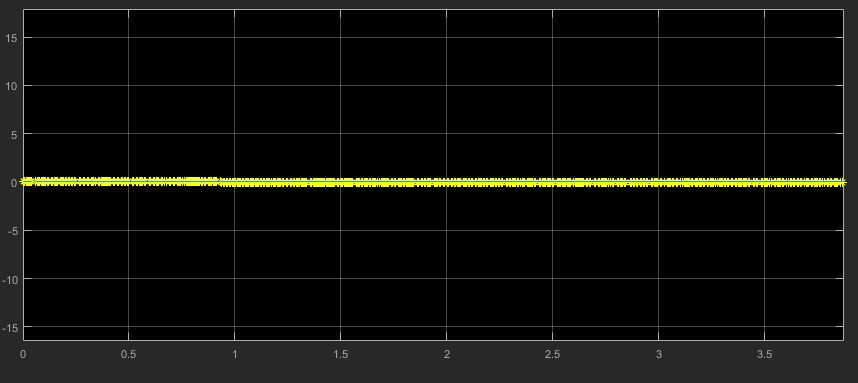
\includegraphics[width=\linewidth]{Undisturbed}
	\caption{Stable system without disturbance}
	\label{fig:4.1}
	\end{center}
	\end{figure}
From figure \ref{fig:4.1} it can be seen that under optimal conditions the system is perfectly stable. However, as it is possible to balance the arm in this position without the motor being driven this is not a difficult state to maintain. In figure \ref{fig:4.2} the state the arm returns to when removed from this base state is shown.
	\begin{figure}[h!]
	\begin{center}
	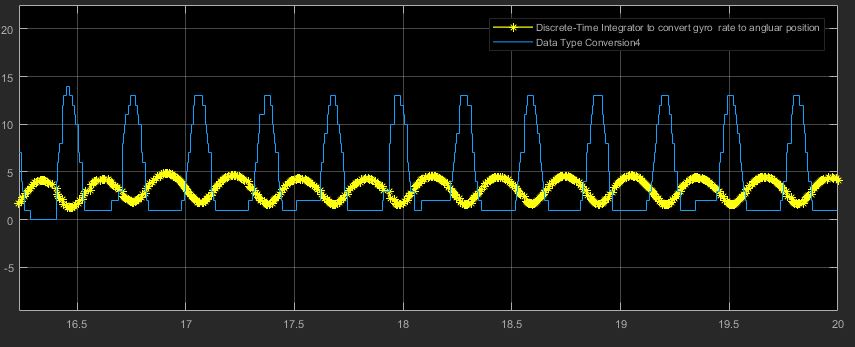
\includegraphics[width=\linewidth]{Ocilation}
	\caption{Return state after disturbance}
	\label{fig:4.2}
	\end{center}
	\end{figure}
While the oscillation was not expected the arm is able to maintain this state indefinitely and can therefore be considered to have remained upright.

        \subsection{Assessment of design criteria}\label{subsec:assessment}
            \subsubsection{Regulation and Disturbance Rejection}
	\begin{figure}[h!]
	\begin{center}
	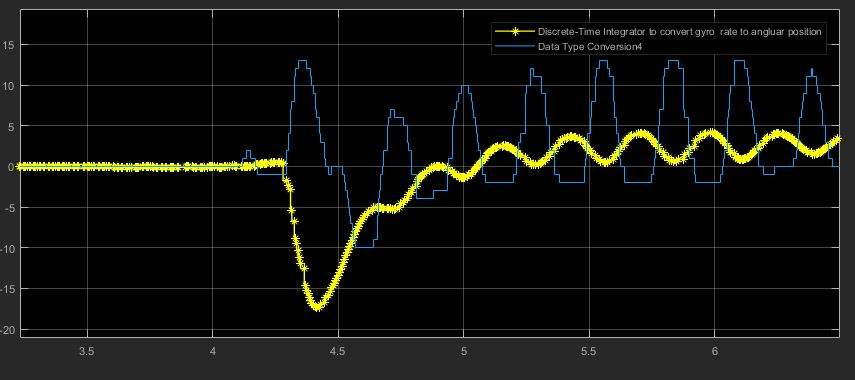
\includegraphics[width=\linewidth]{ImpulseDisturbance}
	\caption{Impulse response}
	\label{fig:4.3}
	\end{center}
	\end{figure}
Figure \ref{fig:4.3} demonstrates the systems ability to recover from an impulse disturbance. As previously mentioned it does not recover from the oscillation, although it is able to maintain the upright position this criterion was considered fulfilled.

	\begin{figure}[h!]
	\begin{center}
	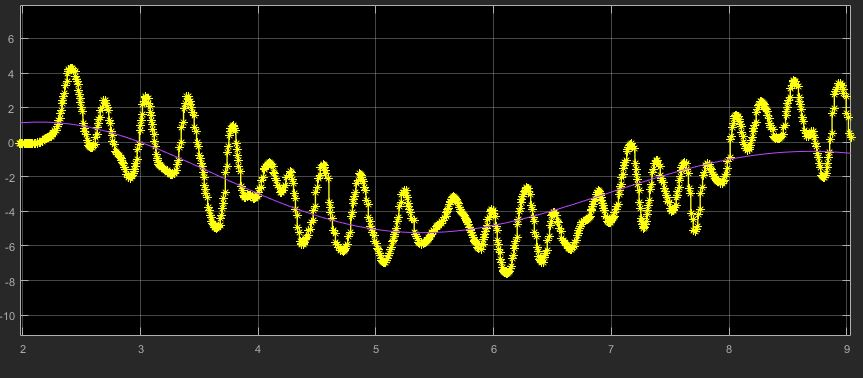
\includegraphics[width=\linewidth]{Steering}
	\caption{Steering resposnce}
	\label{fig:4.4}
	\end{center}
	\end{figure}
For the case of the system in steering mode in figure \ref{fig:4.4} the result is not so clear. While the high frequency oscillation did not present a problem there also a much lower frequency oscillation that, when compared with the steering angle in figure \ref{fig:4.5}, can be seen to be related.

	\begin{figure}[h!]
	\begin{center}
	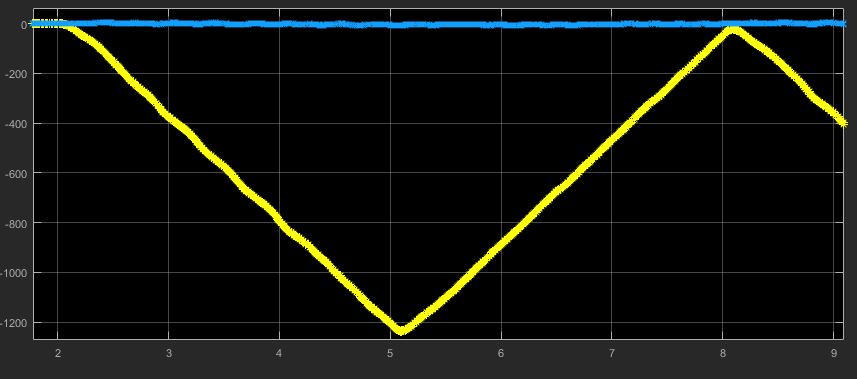
\includegraphics[width=\linewidth]{SteeringWheels}
	\caption{Steering wheel angle}
	\label{fig:4.5}
	\end{center}
	\end{figure}
While it may appear that were the turning to continue the system may fail, it can be seen this is not the case in figure \ref{fig:4.6}. Ignoring the high frequency noise, a lower frequency oscillation can be seen opposing the movement of the arm. From this it can be inferred that were the steering to continue then the system would remain an equilibrium where the centripetal force is balanced by the motor.
	\begin{figure}[h!]
	\begin{center}
	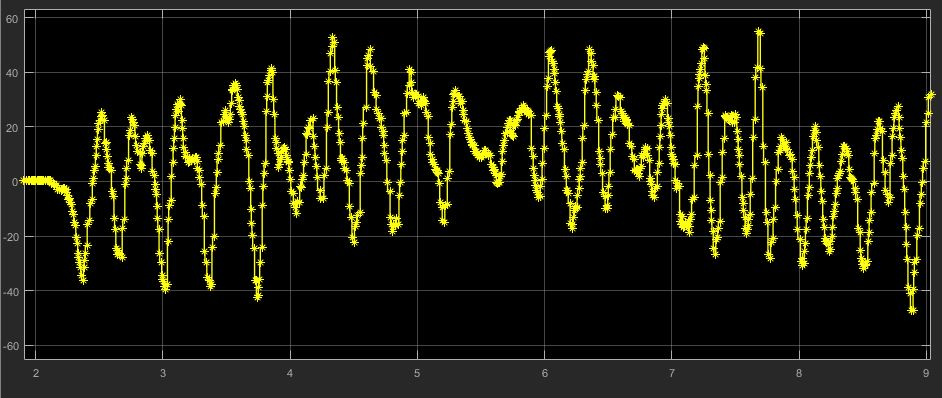
\includegraphics[width=\linewidth]{SteeringVoltage}
	\caption{Motor Driving Voltage}
	\label{fig:4.6}
	\end{center}
	\end{figure}

            \subsubsection{Phase Margin}
Unfortunately, the phase margin could not be shown to be 40$^\circ$. Adding a delay in the system corresponding to 40$^\circ$ at the critical frequency was the method used to test this, however, this resulted in the motor voltage repeatedly saturating and very erratic behaviour. This was due to the fact the maximum force that could be delivered by the motor was not taken into account during the design stage, and as such some boundary cases that may have appeared stable are not reliably so in practice.
	\subsubsection{Bandwidth}
The bandwidth requirement could also not be shown to be fulfilled, however, this was due to an inability to test it rather than because it necessarily wasn’t. The method of testing this would have been to introduce an 50rad/s signal and observe that its magnitude was reduced by more than $\sqrt{2}$. The issue was that the background oscillation of the system either overwhelmed the response for low disturbance magnitudes, or that the motors force limitation would cause the entire system to fail at high magnitudes. As such this criterium could not be verified one way or the other.

        \subsection{Comparison against simulated system}\label{subsec:comp}

	\begin{figure}[h!]
	\begin{center}
	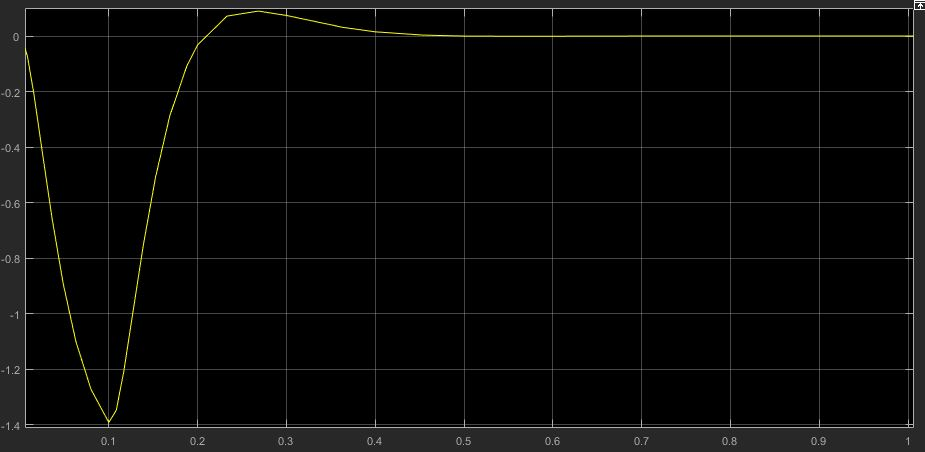
\includegraphics[width=\linewidth]{ImpulseSim}
	\caption{Simulated impulse response}
	\label{fig:4.7}
	\end{center}
	\end{figure}
Figure \ref{fig:4.7} shows the predicted impulse response of the system, and when compared to figure \ref{fig:4.3} several differences can be observed. Most immediately the oscillation present in the system is absent from the model. In addition, it is clear the system is significantly more damped than the model as on returning to steady state the system displays no overshoot and is significantly slower to do so.

There are several reasons this might be the case. The damping effect is likely primarily due to the unmodeled limitations of the motor rather than any real damping. The motor is unable to apply the full expected force that is applied in the model and this results in a damping like effect when the controller voltage saturates.

The oscillation on the other hand is likely caused by the assumptions made during the modelling. Namely the assumption that the motor is completely fixed. In reality it could be seen that the motor was able to shift in the robot, and in addition the entire robot would shift with the pendulum. This added motion was not accounted for and likely the primary reason for the oscillation although there were doubtless other contributing factors.

    \section{Conclusion}\label{sec:con}

While we were unable to demonstrate that all of the criteria discussed in \ref{sec:design} were met, we were able to demonstrate through experiment and calculation that the system is robust and stable. Furthermore we analysed and discussed the shortcomings of our control system, and why the realised system behaves differently to the modelled one.

Improvements could certainly be made to the model in order to better fulfil the design criteria. However better modelling the system would exponentially increase the mathematical complexity of the problem, and as such further experimentation my be the best way to find an improved model.


\end{document}
